\section{Architecture}
To provide a contemporary setup for the decentral and web-based game we have chosen a architecture which will be described in this section.

\begin{figure}[h!]
  \centering
  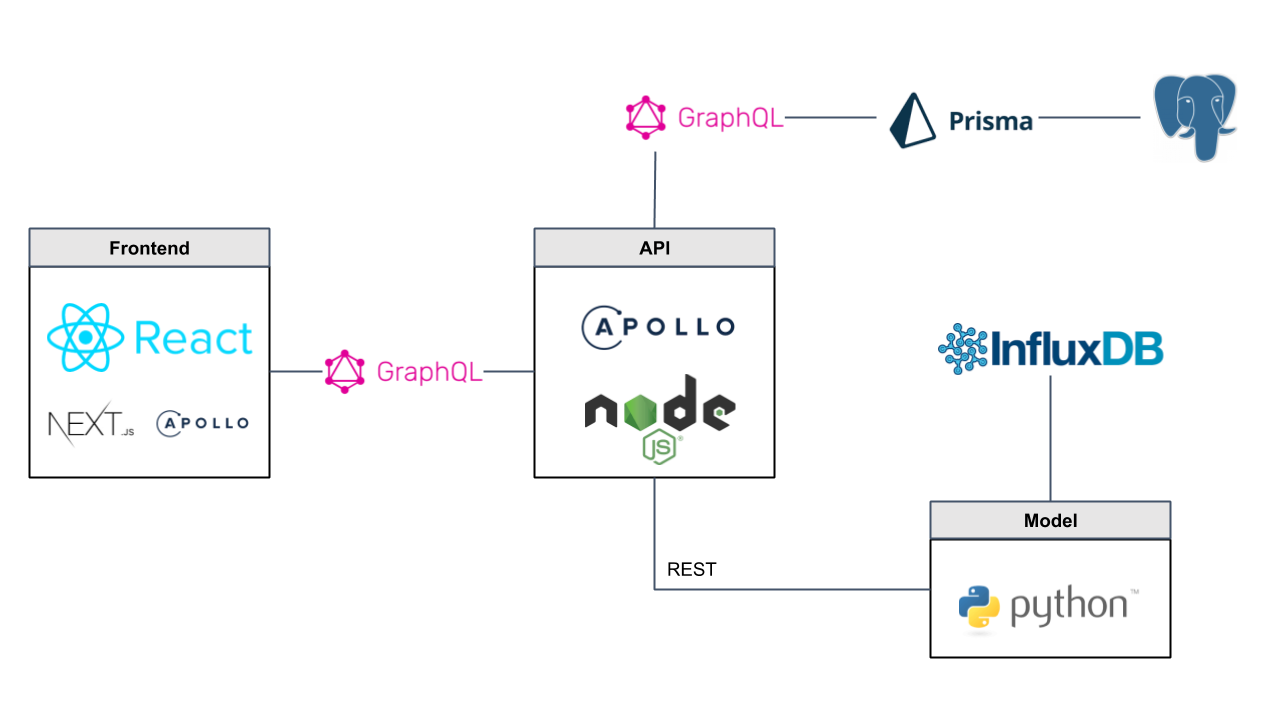
\includegraphics[scale=0.45]{img/architecture.png}
  \caption{PFM game architecture}
\end{figure}


\subsection{Frontend}
\begin{itemize}
  \item Frontend structured as a single-page web application
  \subitem Contrary to native windows application of old game
  \item Allows for effortless setup and requires no manual data transfer
  \subitem Based on the ReactJS and NextJS Javascript Frameworks
\end{itemize}

\subsection{GraphQL}
\begin{itemize}
  \item Declarative data fetching
  \subitem Code snippet (request and response)
  \subitem Backbone for all networking between all application services (except model)
\end{itemize}

\subsection{API / Prisma}
\begin{itemize}
  \item NodeJS backend that serves a single GraphQL API endpoint
  \item Handles authentication and authorization as well as all communications with the model endpoint
  \item Talks to the prisma database access layer for data persistence
\end{itemize}

\subsection{Model}
All calculations of the simulation are performed in a python-model which interacts with the time series data stored on an InfluxDB. A Restful service fetches the data from the model.

\begin{itemize}
  \item Python market and business model (as described in chapter 5)
  \subitem Raw logic and calculations as given by several excel files
  \item Publishes a REST API based on the Falcon framework that can be accessed for different use cases like:
  \subitem Fetching a list of available assets for a certain time period
  \subitem Computing the team scores and results given their decisions and a time period
\end{itemize}

\subsection{Simulation}
\begin{itemize}
  \item Python service that handles time series hydration from the Datastream API as well as sector portfolio construction and new period simulations
  \item Main codebase was constructed by another student during his master thesis on time series simulation. We extended it with an API and additional functionality for the purposes of the game, as well as a more efficient replacement for the data hydration part. The simulation was specifically constructed for the purposes of this game and is planned to be integrated deeply into the portfolio game.
  \item We also handle the infrastructure setup and deployment procedures (''DevOps'') as part of our collaboration.
  \item As this part is described in the thesis of the respective student, we do not go into any further detail regarding his part.
\end{itemize}

\subsection{Continious development}
